\setcounter{chapter}{11}
\chapter{Cinétique Chimique}

\section{Rappels de 1ère sur l'oxydoréduction}
\subsection{Oxydant/Réducteur}
\begin{itemize}
	\item Un oxydant est une espèce chimique capable de \trou{capter} un ou plusieurs électrons.
	\item Un réducteur est une espèce chimique capable de \trou{céder} un ou plusieurs électrons.
	\item De manière générale on peut écrire cet échange sous la forme d'une demi-équation électronique: $$\boxed{Ox + n\cdot e^- = Red}$$
\end{itemize}
\etiquette{Exemples} $Cu^{2+}/Cu$ ; $I_2/I^-$ ; $H^+/H_2$ sont des couples redox. Ecrire les demi-équations électroniques associées à chaque couple.
\begin{align*}
	Cu^{2+} + \trou{2e-} &= Cu\\
I_2 + \trou{2e^-} &= \trou{2I^-}\\
\trou{2H^+} +\trou{ 2e^-} &= \trou{H_2}
\end{align*}

\blocrouge{Méthodes pour écrire les demi-équations}{
\begin{enumerate}
	\item Equilibrer les atomes autres que\trou{ O et H}.
	\item Equilibrer O en ajoutant des \trou{molécules d'eau}.
	\item Equilibrer H en ajoutant des ions \trou{$H^+$}.
	\item Ajouter des électrons pour \trou{équilibrer les charges électriques}
\end{enumerate}}

\etiquette{Application} Ecrire les demi-équations électroniques associées aux couples suivant: $O_2/H_2O$ ; $H_2O_2/H_2O$ ; $O_2/H_2O_2$ ; $MnO_4^-/Mn^{2+}$.
\newpage
\subsection{Equation chimique d'une réaction d'oxydoréduction}
\blocrouge{Méthode} {
\begin{enumerate}
	\item Repérer les couples.
	\item Ecrire les demi-équations dans le sens où elles se font (voir exemple) 
	\item Vérifier que chaque demi-équation échange le même nombre d'électrons. Si ce n'est pas le cas, multiplier par des coefficients appropriés.
	\item Additionner les demi-équations. Les électrons doivent se neutraliser.
	\item Vérifier que l'équation obtenue est équilibrée en termes d'atomes et de charges.
\end{enumerate}
}

\etiquette{Exemples} On fait réagir le fer Fe et le dichlore $C\ell_2$. Voici les couples redox: $Fe^{3+}/Fe$ et $C\ell_2 / C\ell^-$.
\begin{align*}
 \trou{ 2\text{Fe}} &\rightarrow \trou{2\text{Fe}^{3+}} +\trou{ 6e^-} \\
    \trou{3}\text{Cl}_2 + \trou{6}e^- &\rightarrow \trou{6\text{Cl}^- }\\
    \hline
    \trou{2\text{Fe} + 3\text{Cl}_2 }&\rightarrow \trou{2\text{Fe}^{3+} + 6\text{Cl}^-}
\end{align*}


\section{Transformations lentes et rapides}
\subsection{Transformations rapides}
\etiquette{Critère}
Une transformation est rapide lorsque à nos yeux elle semble instantanée. C'est à dire que les réactifs se transforment en produits en moins d'une seconde.

\etiquette{Exemples:}
\begin{itemize}
	\item Les explosions sont des réactions très rapides.
	\item Les réactions qui forment des précipités sont très rapides. \\
Réaction entre les ions chlorures et les ions argents pour former le chlorure d'argent

\end{itemize}

Schéma + équation de la réaction

\vspace{3cm}

\subsection{Transformations lentes}
Les réactions qui ne sont pas rapides sont lentes...

\etiquette{Exemple}

coucher de soleil du chimiste

\subsection{Comment suivre l'évolution des réactions lentes ?}

\etiquette{Problème} Comment mesurer la quantité de matière de produit apparu à chaque instant pendant que la réaction se fait ?

\etiquetterouge{3 techniques à relier aux TP}
\begin{enumerate}
	\item Si le produit ou le réactif est coloré: on suit l'absorbance avec un spectrophotomètre.
	\item Si le produit ou un réactif est un ion: on suit la conductivité avec un conductimètre.
	\item On prélève un échantillon du milieu réactionnel et on effectue un titrage. (voir chapitre Titrages)	
\end{enumerate}

\section{Comment modifier la vitesse d'une réaction ?}
\subsection{Facteurs cinétiques}

\blocrouge{Définitions}{
\begin{itemize}
	\item Un facteur cinétique est une grandeur qui a une influence sur la durée de la réaction chimique.
	\item Il existe 2 facteurs cinétiques: 
		\begin{enumerate}
			\item \trou{La température: Plus la température est élevée plus la réaction est rapide.}
			\item \trou{La concentration: Plus la concentration des réactifs est grande plus la réaction est rapide.}
		\end{enumerate}
\end{itemize}
}
\subsection{Mise en évidence expérimentale}
Voir TP Facteurs Cinétiques


\subsection{Catalyser une réaction}
\blocrouge{Définition}{
Un catalyseur est une espèce chimique qui diminue la durée d'une transformation chimique. Il ne modifie pas \trou{l'état final du système}.
}

\etiquette{Conséquences et propriétés}
\begin{itemize}
	\item Un catalyseur ne figure pas dans l'équation chimique de la réaction.
	\item La quantité de produit formé ne dépend pas de la présence d'un catalyseur.
	\item Le catalyseur n'est pas \trou{consommé} et se retrouve intégralement à la \trou{ fin } de la réaction.
	\item Un catalyseur est en général spécifique à une réaction chimique.
\end{itemize}

\etiquette{Effet de la présence d'un catalyseur}
L'eau oxygénée réagit sur elle même car l'eau oxygénée est à la fois un oxydant et un réducteur. 

Les couples oxydant/réducteur impliqués sont :
\begin{align*}
    \text{O}_2 / \text{H}_2\text{O}_2 \\
    \text{H}_2\text{O}_2 / \text{H}_2\text{O}
\end{align*}

Écrire les Demi-Équations d'Oxydoréduction :

Pour \(\text{O}_2 / \text{H}_2\text{O}_2\) (réduction) :
\begin{align*}
   \text{H}_2\text{O}_2 &=  \text{O}_2 + \trou{2\text{H}^+} + \trou{2}e^-
\end{align*}

Pour \(\text{H}_2\text{O}_2 / \text{H}_2\text{O}\) (oxydation) :
\begin{align*}
    \text{H}_2\text{O}_2 +\trou{ 2\text{H}^+} +\trou{ 2e^-} &= \trou{2}\text{H}_2\text{O} 
\end{align*}

En additionnant membre à membre, on obtient la réaction de Dismutation de l'eau oxygénée: $$2H_2O_2 \longrightarrow 2H_2O + O_2 $$
Différentes catalyses possibles pour cette réaction :
\begin{enumerate}
	\item utilisation de Pt (catalyse hétérogène)
	\item solution de $Fe^{2+}$ (catalyse homogène)
\end{enumerate}


%\newpage
\section{Vitesse volumique}
\subsection{Situation}
La réaction entre les ions peroxodisulfate $S_2O_8^{2-}$ et les ions iodures $I^-$ est lente. Elle produit du diiode (orange) et des ions sulfate incolore selon:
$$S_2O_8^{2-}+2I^-\longrightarrow 2 SO_4^{2-}+I_2$$ 
\begin{minipage}{0,45\linewidth}
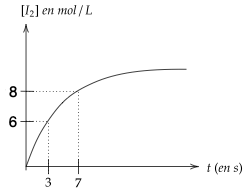
\includegraphics[scale=1]{figures/cinetique/fig_cinetique1_v2}
\end{minipage}
\begin{minipage}{0,6\linewidth}

Ci-contre, la courbe d'évolution de la concentration du diiode dans le mélange réactionnel au cours du temps.\\
Le diiode étant une espèce colorée, cette courbe a pu être obtenue par spectrophotométrie.
\end{minipage}

\etiquette{Estimation de la vitesse volumique d'apparition de $I_2$}
\begin{itemize}
	\item Entre t=3 s et t=7 s il s'est écoulé une durée de \trou{7-3 = 4 s}.
	\item Pendant cette durée, la concentration du diiode a augmenté de: \trou{10-8=2 mol/L}
	\item On peut donc dire qu'en 4 s la concentration a augmenté de 2 mol/L.
	\item Cela correspond à une vitesse volumique moyenne de $$V_{app}(I_2) \approx \frac{2 \: mol/L}{4\:s}=0,5\:mol.L^{-1}.s^{-1}$$
\end{itemize}

\etiquetterouge{Attention} Nous allons maintenant calculer la vitesse volumique instantanée en reprenant l'idée de vitesse instantanée vue en mécanique. C'est cette définition et la technique qui suit que vous devez retenir.
\subsection{Généralisation et définition rigoureuse de la vitesse volumique}
\includegraphics{figures/cinetique/fig_cinetique2}


$$V_{app}(X)=\dfrac{[X](t+\Delta t)-[X](t)}{\Delta t}$$

Si $\Delta t$ tend vers 0, alors la vitesse d'apparition moyenne tend vers la vitesse d'apparition instantanée.
$$\lim\limits_{\Delta t \to 0}V_{app}(X)=\lim\limits_{\Delta t \to 0}\dfrac{[X](t+\Delta t)-[X](t)}{\Delta t}$$
\blocrouge{Définition de la vitesse volumique d'apparition}{On note $[X](t)$ la concentration d'un produit $X$ à l'instant t, dans le mélange réactionnel. Entre les instants $t$ et $t+\Delta t$ la concentration de $X$ augmente. Pour rendre compte de la vitesse la concentration de $X$ augmente, on calcule sa vitesse volumique d'apparition :$$V_{app}(X)=\trou{\frac{d[X]}{dt}}$$
\begin{itemize}
	\item $[X]$ est la concentration en mol/L
	\item t le temps en s
	\item $V_{app}$ en $mol.L^{-1}.s^{-1}$
\end{itemize}}

\newpage
\subsection{Technique pour calculer une vitesse volumique d'apparition}

\blocrouge{Technique}{La vitesse volumique d'apparition est égale \trou{au coefficient directeur de la tangente à la courbe. }}

\etiquette{Exemple}

\begin{minipage}{0,45\linewidth}
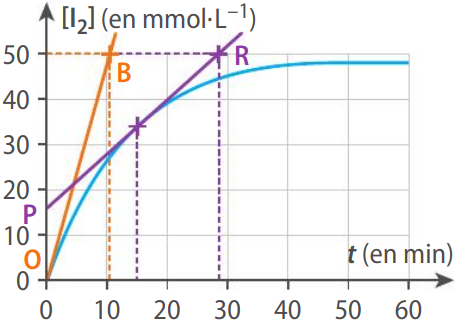
\includegraphics[scale=0.5]{figures/cinetique/fig_3}
\end{minipage}
\begin{minipage}{0,45\linewidth}
Déterminer les vitesses volumiques d'apparition de $I_2$ au temps t=0 et au temps t=15 min. Commenter.
\end{minipage}

\vspace{8cm}
\subsection{Vitesse volumique de disparition}
Soit R un réactif dont on souhaite connaître la vitesse de disparition. En utilisant le même raisonnement que pour la vitesse d'apparition, on va calculer s'intéresser à la dérivée de sa concentration $\dfrac{d[R]}{dt}$.

La vitesse de disparition est positive.  $[R](t)$ est décroissante donc sa dérivée est négative. C'est pourquoi, on ajoute un signe - pour le calcul de la vitesse de disparition.

\blocrouge{Définition}{
Soit $X$ un réactif consommé lors d'une réaction, sa vitesse volumique de disparition est donnée par
$$V_{disp}(X)=-\frac{d[X]}{dt}$$
\begin{itemize}
	\item $[X]$ est la concentration en mol/L
	\item t le temps en s
	\item $V_{disp}$ en $mol.L^{-1}.s^{-1}$
\end{itemize}}
 
 
\section{Loi de vitesse d'ordre 1}
\subsection{Contexte}
Considérons une réaction ayant pour équation :
\begin{center}
$ a A + b B \longrightarrow c C$
\end{center}
La vitesse de disparition du réactif A s'écrit alors : $$V_{disp}(A)=\trou{-\dfrac{d[A]}{dt}}$$


\blocrouge{Définition}{
Une réaction chimique suit une loi de vitesse d'ordre 1 si à tout instant t, la vitesse volumique de disparition est proportionnelle à la concentration en A, c'est à dire si :\\
$$V_{disp}(A)=\trou{k[A](t)=-\dfrac{d[A]}{dt}}$$ où $k$ est une constante.
}


\etiquette{Unités}
Retrouver par analyse dimensionnelle l'unité de k.\\
\vspace{2cm}

\etiquette{Aspect mathématique: Equation différentielle}
Lorsque la loi de vitesse est d'ordre 1: et donc : $$\trou{\dfrac{d[A]}{dt}+k[A](t)=0}$$ On montre (voir annexe) que l'évolution au cours du temps de la concentration de A suit une loi exponentielle décroissante qui s'écrit: $$[A](t) = [A]_0 \times e^{-k.t}$$
\newpage
\section{Temps de demi-réaction}

\blocrouge{Définition}{
Le temps de demi réaction $t_{1/2}$ est la durée au bout de laquelle l'avancement $x(t_{1/2})$ la réaction a atteint  la moitié de la valeur de l'avancement final $x_f$. $$x(t_{1/2})=\frac{x_f}{2}$$
}

\etiquette{Détermination Graphique}

\begin{minipage}{0,45\linewidth}
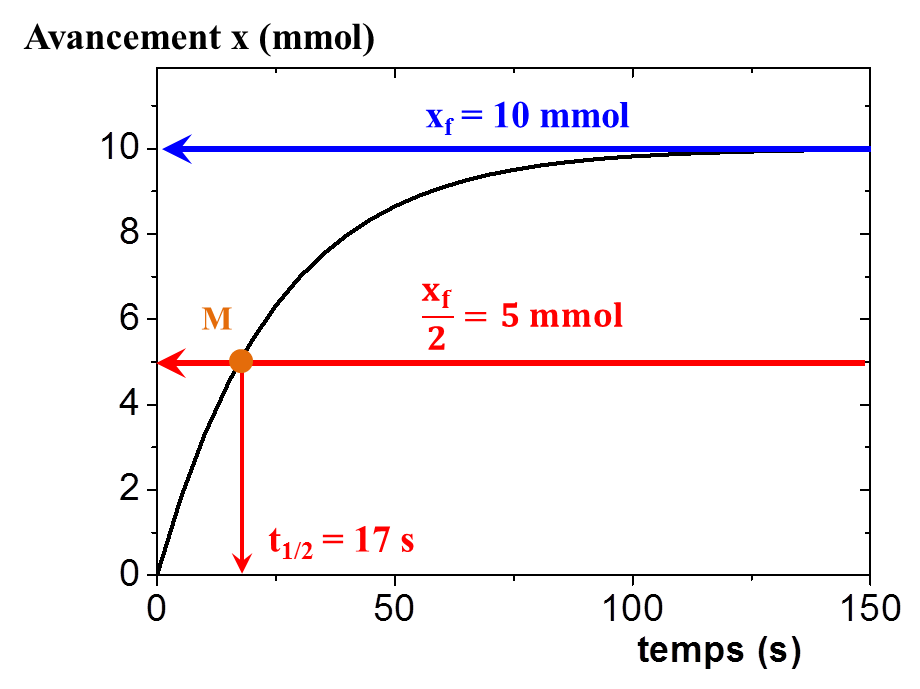
\includegraphics[scale=.5]{figures/cinetique/demi_reaction.png} 
\end{minipage}
\begin{minipage}{0,45\linewidth}
Technique: Repérer la valeur de l'avancement maximal, calculer $x_f /2$. Trouver le point de la courbe dont l'ordonnée est $x_f /2$. Son abscisse est le temps de demi-réaction
\end{minipage}

Autre type de graphique: Représentation de la concentration d'un réactif au cours du temps ou de l'absorbance d'un réactif au cours du temps.

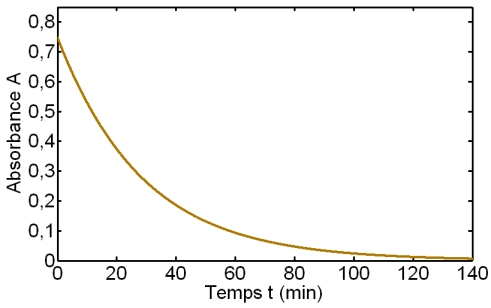
\includegraphics[scale=.45]{figures/cinetique/fig_4.jpg}


\section{Comment tester si une loi de vitesse est d'ordre 1 ?}
\subsection{3 Techniques à connaître}
\etiquette{Technique 1: En utilisant t1/2}\\
On réalise plusieurs expériences en faisant varier les concentrations initiales $[A]_0$. Si le temps de demi-réaction ne change pas d'une expérience à une autre alors la loi de vitesse est d'ordre 1.Faire \textbf{Ex 11 p 86}

\etiquette{Technique 2: Vitesse proportionnelle à la concentration}

Si la vitesse de disparition d'une réactif est proportionnelle à la concentration de ce réactif $$V_{disp}(A)=\trou{k[A](t)}$$ Alors la loi de vitesse est d'ordre 1. \textbf{Ex 13 p 86} (estimer les vitesses à partir des cordes de la courbe)

\etiquette{Technique 3: Modélisation de l'évolution de $[A](t)$}

Pour une loi de vitesse d'ordre 1, on a $[A](t)=[A]_0e^{-kt}$.\\ On peut vérifier cette relation par une modélisation de $[A(t)]$ en utilisant Regressi ou un programme Python. 

Voir \textbf{2022-Centres Etrangers-J1-ExoC-Sujet-Cinetique-AcBase}


\section*{ANNEXES}
\subsection*{Annexe 1: Solution de l'équation différentielle}
Résolution de $\dfrac{d[A]}{dt}= -k[A](t)$
On reconnaît une équation différentielle d'ordre 1. 

\etiquette{Solution Générale}

$[A](t)=Ce^{-k\cdot t}$ où  C une constante est solution de l'équation différentielle.

Vérifiez que c'est bien le cas en injectant cette expression dans l'équation différentielle.

\etiquette{Recherche de C avec une condition initiale}

On sait que à t=0 
\begin{itemize}
	\item la concentration en A est connue: $[A](t=0) = [A]_0$ 
	\item en utilisant la solution générale, on a aussi: $[A](t=0) = C.e^{-k\times 0} = C$
\end{itemize}
Donc $$C =  [A]_0$$
Connaissant $C$, nous pouvons réécrire la solution générale de manière complète.

\etiquette{Conclusion}
$$\boxed{[A](t) = [A]_0 \times e^{-k.t}}$$

\subsection*{Annexe 2}
On prend le logarithme de $[A(t)]$ ce qui donne : \trou{$ln([A](t))=ln([A]_0)-kt$}\\

En traçant le graphe de \trou{ln[A] en fonction du temps}

\subsection*{Interprétation du graphique}
\begin{center}
	\includegraphics[scale=.8]{figures/cinetique/loi_vitesse} 
\end{center}
2 cas possibles: 
\begin{enumerate}
	\item On obtient une droite de coefficient directeur égal à -k : la loi de vitesse est d'ordre 1.
	\item On n'obtient pas une droite, alors l'évolution de la concentration ne suit pas une loi de vitesse d'ordre 1. 	
\end{enumerate}


\blocrouge{A FAIRE}{
\begin{itemize}
	\item Résumé et techniques + quizz: \url{https://youtu.be/NO87Hcyt7OU}
	\item  6,13,14,15,19, 22 et prépa ece p90
	\item  Sujet type BAC: Centres étrangers 2021 sujet 2
\end{itemize}}




 
 %\newpage
 \section{Modélisation microscopique}
 \subsection{Acte élémentaire}
\blocrouge{Définition}{
A l'échelle microscopique, on observe une réaction se déroulant en \trou{une seule étape} $$A+B\longrightarrow C+D$$ cette réaction est appelée \trou{acte élémentaire}.
}


\etiquette{Choc efficace ?}

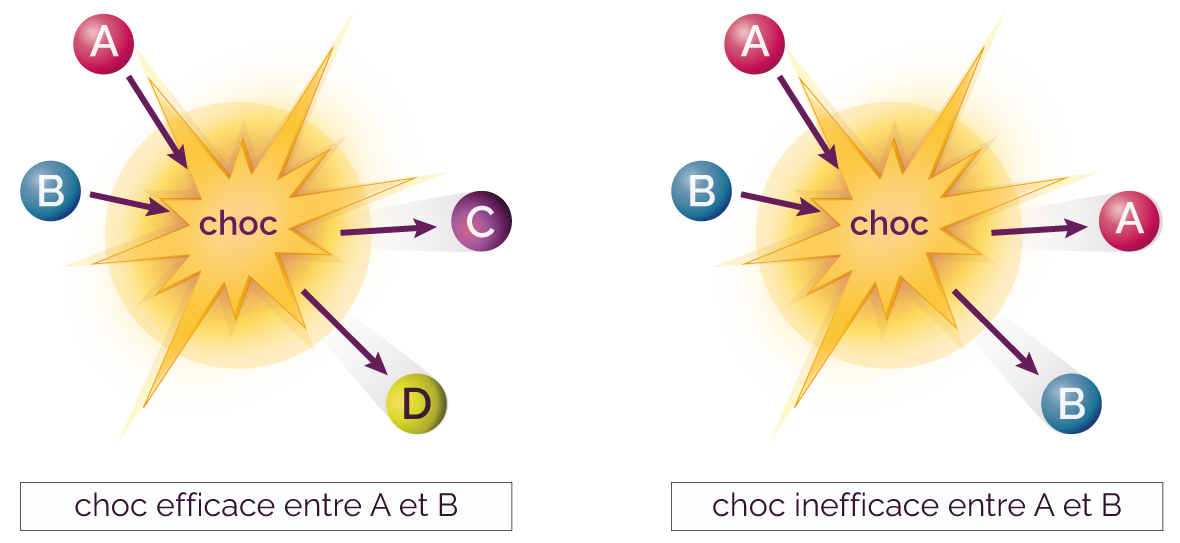
\includegraphics[width=10cm]{figures/cinetique/choc.png}

La simple rencontre des réactifs A et B ne suffit pas à engendrer l'apparition des produits.  Cette rencontre doit se faire sous la forme d'une choc suffisamment violent pour que les liaisons chimiques de A et B se réorganisent pour former les produits C et D. On dit que le choc est \trou{efficace}.

\etiquette{Conséquences}

\begin{itemize}
	\item Plus la température est grande, plus l'efficacité des chocs est \trou{grande} et plus la vitesse de réaction est \trou{grande}.
	\item Plus la concentration d'un réactif est grande, plus les chocs efficaces sont \trou{fréquents}et plus la vitesse est grande.
\end{itemize}
 
\subsection{Mécanisme Réactionnel}
\blocrouge{Définition}{Une réaction chimique peut être décomposée en une \trou{succession d'actes élémentaires}. Cette décomposition forme un \trou{mécanisme réactionnel}.}
 
 \etiquette{Exemple} La réaction entre le chlorométhane et l'ion hydroxyde s'écrit à l'échelle macroscopique: $$CH_3-C\ell + HO^- \longrightarrow CH_3-OH + C\ell^-$$
 Son mécanisme réactionnel, comporte deux actes élémentaires :
 

\begin{alignat*}{2}
    &\textbf{Acte élémentaire 1} \quad \quad \quad &&CH_3-Cl \leftrightharpoons CH_3-C^+ + Cl^- \\
    &\textbf{Acte élémentaire 2} \quad \quad \quad &&CH_3-C^+ + HO^- \leftrightharpoons CH_3-OH \\
    \hline 
    &\textbf{Bilan} \quad &&\trou{CH_3-Cl + HO^- \longrightarrow CH_3-OH + Cl^-}
\end{alignat*}

\blocrouge{Intermédiaire Réactionnel}{Un intermédiaire réactionnel est une espèce chimique qui \trou{apparaît dans un acte élémentaire} et disparaît dans l'acte suivant. Il ne figure pas dans le bilan de la réaction.}

\etiquette{Travail} Repérer dans le mécanisme ci-dessus un intermédiaire réactionnel.

\blocrouge{Repérer un catalyseur !}{Dans un mécanisme réactionnel, le catalyseur est présent dans l'acte 1 et régénéré dans un acte suivant. La présence du catalyseur modifie le mécanisme réactionnel.}

La réaction précédente est maintenant réalisée en présence d'ion iodure $I^-$. Voici le mécanisme réactionnel: 

\begin{alignat*}{2}
    &\textbf{Acte élémentaire 1} \quad \quad \quad &&CH_3-Cl + I^-\leftrightharpoons CH_3-I + Cl^- \\
    &\textbf{Acte élémentaire 2} \quad \quad \quad &&CH_3-C^+ + HO^- \leftrightharpoons CH_3-OH + I^-
    \end{alignat*}

\etiquette{Question}
\begin{enumerate}
	\item Justifier que $I^-$ est un catalyseur
	\item Justifier que la présence du catalyseur ne modifie pas l'équation bilan de la réaction.
\end{enumerate}

\etiquetterouge{Conclusion} L'équation bilan d'une réaction modélise à l'échelle macroscopique la réaction chimique. Le mécanisme réactionnel donne une modélisation microscopique dont les actes élémentaires peuvent mettre en évidence un ou plusieurs intermédiaires réactionnels.
En faisant la somme  des actes élémentaires on retrouve \trou{l'équation bilan.}

\newpage
\section{Formalisme de la flèche courbe}
	\subsection{A quoi ça sert ?}

Afin de justifier les actes élémentaires, on utilise des flèches courbes pour montrer le déplacement des doublets électroniques. La flèche est toujours orientée du site donneur vers le site accepteur de doublet. Elle s'écrit du doublet vers l'atome (cf exemple). La ou les flèches courbes sont toujours côté réactif dans l'acte élémentaire.

\etiquette{Exemple}

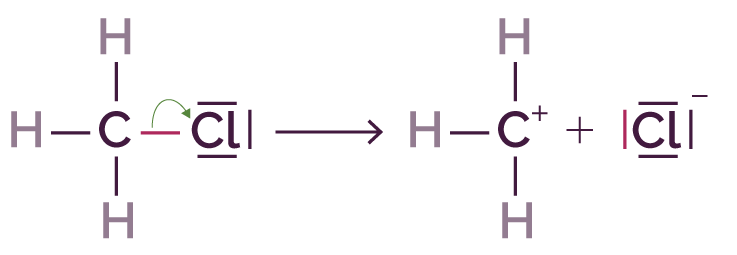
\includegraphics[width=8cm]{figures/cinetique/fleche1.png}

\subsection{Site donneur / Site accepteur}
\etiquette{Site Donneur}

\begin{enumerate}
	\item Atome possédant un doublet liant (cf le C de l'exemple)
	\item Atome possédant un \trou{doublet non liant}
\end{enumerate}

\etiquette{Site Accepteur}
\begin{enumerate}
	\item Atome ou ion possédant une lacune (comme l'ion $H^+$ ou l'atome de bore $B$).
	\item Atome possédant une charge formelle.
	\item  Atome avec une charge partielle (liaison polarisée)
\end{enumerate}

\etiquette{Extrait BAC 2018 Afrique}

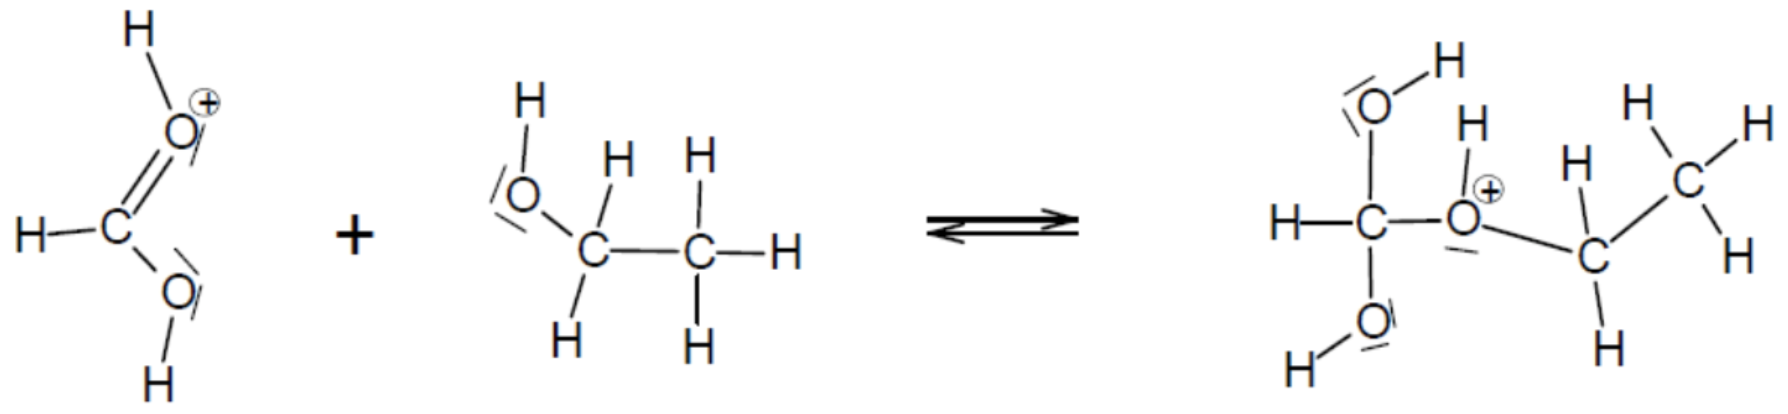
\includegraphics[width=13 cm]{figures/cinetique/sites.png}
 \begin{enumerate}
 	\item Identifier les sites donneurs et le site accepteur mis en jeu lors de l'acte élémentaire.
 	\item Représenter par des flèches courbes les déplacements de doublets électroniques.
 \end{enumerate}
 
 \etiquette{Application directe}
 
 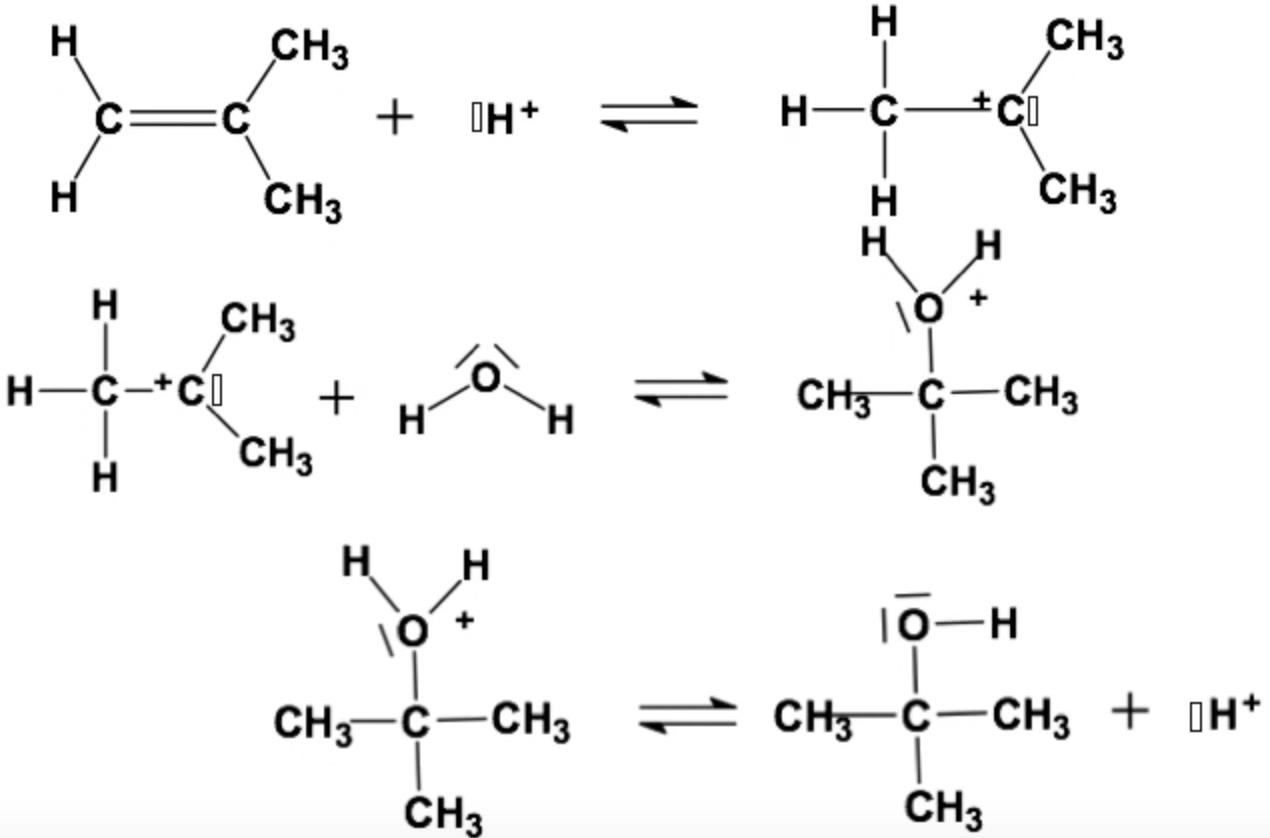
\includegraphics[width=12cm]{figures/cinetique/mecanisme.png}
 
 \begin{enumerate}
 	\item Retrouver l'équation de la réaction modélisée par le mécanisme réactionnel fourni.
 	\item Identifier les intermédiaires réactionnels.
 	\item Quel est le rôle de l'ion hydrogène dans ce mécanisme ? Justifier votre réponse.
 	\item Pour chaque acte élémentaire, représenter les flèches courbes.
 \end{enumerate}

 \etiquette{EXERCICES à faire}
  Dans ton livre: 
  \begin{itemize}
  	\item Vérifier vos réflexes: 5, 7 , 9 p 103
  	\item Pour s'entrainer et faire les classiques: 11 ou 12 p 105 ; 19 p 107
  	\item Muscler son jeu: 20, 21 p 108
  \end{itemize}
 \etiquette{Vidéo}
 Pour revoir en détail l'électronégativité et le déplacement de doublet: 
 \url{https://youtu.be/ETVjaxuNWn8?si=dI-H-Vo9Lh_SBK4E}